
\chapter{Root Locus}
\label{ch:root_locus}

\begin{quote}
\textit{``The root locus method is probably the most powerful tool available for control system design and analysis.''} --- Walter R. Evans, 1950
\end{quote}

\vspace{1em}

The root locus technique stands as one of the most elegant and intuitive methods in control system analysis. Developed by Walter R. Evans in 1948, this graphical method provides deep insight into how closed-loop system dynamics change as a design parameter---typically the loop gain $K$---varies from zero to infinity. Understanding root locus is essential for any control engineer, as it bridges the gap between mathematical analysis and practical design intuition.

%=============================================================================
\section{Historical Motivation: The Genesis of Root Locus}
\label{sec:history}
%=============================================================================

\subsection{The Challenge of Aircraft Autopilot Design}

In the years following World War II, the aerospace industry faced unprecedented challenges in automatic flight control. Aircraft were becoming faster, more complex, and increasingly difficult for human pilots to control manually in all flight conditions. The development of reliable autopilot systems became a critical priority, and engineers at North American Aviation found themselves at the forefront of this challenge.

Walter R. Evans, a young engineer working at North American Aviation in Los Angeles, was tasked with designing autopilot systems for advanced aircraft. The fundamental problem he faced was deceptively simple to state but extraordinarily difficult to solve: \textit{How does one choose the gain $K$ in a feedback control system to achieve desired closed-loop behavior?}

Consider a typical unity feedback control system with open-loop transfer function $G(s)$. The closed-loop transfer function is:
\begin{equation}
T(s) = \frac{KG(s)}{1 + KG(s)}
\label{eq:closed_loop}
\end{equation}

The closed-loop poles---the roots of the characteristic equation $1 + KG(s) = 0$---completely determine system stability and transient response. But here lay the challenge: for any given value of $K$, finding these roots required solving a polynomial equation, often of high order.

\subsection{The Pre-Computer Era: Tedium and Trial}

Before electronic computers became widely available, solving polynomial equations was a laborious manual process. Engineers in the 1940s relied on several techniques, each with significant limitations. Direct calculation required applying various root-finding algorithms by hand, and for a fifth-order characteristic polynomial, this process could take hours for a single value of $K$. The Routh-Hurwitz analysis method could determine stability without finding exact pole locations, but it provided no information about transient response characteristics. Frequency response methods such as Bode and Nyquist plots offered valuable stability insights but did not directly reveal pole locations.

The iterative design process was painfully slow. An engineer might select a trial value of $K$, then spend several hours solving the characteristic equation by hand, only to discover that the resulting poles did not provide acceptable response characteristics. This would necessitate guessing a new value of $K$ and repeating the entire calculation. For a typical autopilot design requiring optimization of multiple parameters, this process could consume weeks of engineering time.

\subsection{Evans' Revolutionary Insight}

\begin{historicalbox}[Walter R. Evans and the Root Locus Method]
Walter R. Evans (1920--1999), a young engineer at North American Aviation in Los Angeles, revolutionized control system design in 1948. His breakthrough came from asking a fundamentally different question: rather than ``Where are the poles for this specific $K$?'' he asked ``Where can the poles possibly be as $K$ varies over all positive values?'' Evans published his method in ``Graphical Analysis of Control Systems'' (1948) and ``Control System Synthesis by Root Locus Method'' (1950). He received the AIEE's Lamme Medal in 1957 and IFAC's Nichols Medal in 1987 for this transformative contribution that reduced weeks of hand calculations to minutes of geometric construction.
\end{historicalbox}

Walter Evans' breakthrough came from a fundamental shift in perspective.

This reframing transformed the problem from repeated point calculations to a single geometric construction. Evans recognized that the locus of possible pole locations could be sketched directly from the open-loop pole and zero locations, without solving the characteristic equation even once.

His key observations revealed a beautiful geometric structure underlying the problem. At $K = 0$, the closed-loop poles coincide with the open-loop poles. As $K \to \infty$, the closed-loop poles migrate toward the open-loop zeros, or toward infinity along specific asymptotic directions when there are more poles than zeros. Most importantly, Evans recognized that the paths followed by the poles obey precise geometric rules derivable from the angle and magnitude conditions, making it possible to sketch the complete locus without solving any equations.

\begin{figure}[H]
\centering
\begin{tikzpicture}[scale=1.2]
    % Axes
    \draw[->,thick] (-4.5,0) -- (2,0) node[right] {$\sigma$};
    \draw[->,thick] (0,-3) -- (0,3) node[above] {$j\omega$};

    % Open-loop poles
    \filldraw[blue] (-3,0) circle (3pt) node[below=5pt] {$p_1$};
    \filldraw[blue] (-1,1) circle (3pt) node[above right] {$p_2$};
    \filldraw[blue] (-1,-1) circle (3pt) node[below right] {$p_3$};

    % Open-loop zero
    \draw[red,thick] (-2,0) circle (4pt);
    \node[red] at (-2,-0.4) {$z_1$};

    % Root locus branches (simplified illustration)
    \draw[thick,blue!70!black,->] (-3,0) -- (-2.1,0);
    \draw[thick,blue!70!black,decoration={markings, mark=at position 0.6 with {\arrow{>}}},postaction={decorate}]
        (-1,1) .. controls (0.5,1.5) and (0.5,2.5) .. (-0.5,2.8);
    \draw[thick,blue!70!black,decoration={markings, mark=at position 0.6 with {\arrow{>}}},postaction={decorate}]
        (-1,-1) .. controls (0.5,-1.5) and (0.5,-2.5) .. (-0.5,-2.8);

    % Labels
    \node[blue] at (-3.5,0.4) {$K=0$};
    \draw[->,thin] (-3.3,0.3) -- (-3.1,0.1);

    \node at (1.2,2.5) {$K \to \infty$};

    % Title
    \node at (-1,-3.5) {\textbf{Root locus showing pole migration as $K$ increases}};
\end{tikzpicture}
\caption{Conceptual illustration of Evans' insight: closed-loop poles trace continuous paths from open-loop poles ($K=0$) toward zeros or infinity ($K \to \infty$).}
\label{fig:evans_insight}
\end{figure}

Evans published his groundbreaking work in 1948 in the paper ``Graphical Analysis of Control Systems'' in the \textit{Transactions of the AIEE}. He followed this with a more comprehensive treatment in 1950, ``Control System Synthesis by Root Locus Method,'' which established the complete set of construction rules still used today.

\subsection{Impact on Control Engineering Practice}

The root locus method revolutionized control system design. What had previously required days of calculation could now be accomplished in minutes with a pencil, paper, and a simple protractor called a ``Spirule'' (which Evans himself helped design). Engineers could now visualize the complete range of possible closed-loop behaviors at a glance, immediately identify gain ranges that would cause instability, and select gains to achieve desired damping ratios and natural frequencies. Perhaps most powerfully, they could understand how adding compensator poles and zeros would reshape the locus, enabling systematic compensator design.

The method spread rapidly through the control engineering community. By the mid-1950s, root locus had become a standard topic in control systems curricula, and it remains so today. Evans received the AIEE's Lamme Medal in 1957 and the IFAC's inaugural Nichols Medal in 1987 for his contributions.

\subsection{Relevance in the Computer Age}

One might question whether a graphical method developed for hand calculation remains relevant when modern computers can instantly solve characteristic equations of any order. The answer is an emphatic yes, for several reasons. First, root locus provides unparalleled design intuition into how system dynamics depend on parameters; a designer who understands root locus can predict how modifications will affect performance without running simulations. Second, adding poles and zeros to reshape the root locus is a powerful compensator design technique that is best understood through the geometric interpretation. Third, root locus reveals how pole locations change with parameter variations, providing immediate robustness and sensitivity information. Finally, learning root locus develops spatial intuition about polynomial roots that benefits all areas of dynamic systems analysis.

While we now use MATLAB's \texttt{rlocus} command or Python's \texttt{control} library rather than Spirules and drafting tables, the underlying principles Evans discovered remain the foundation of modern control design practice.

%=============================================================================
\section{Modern Applications}
\label{sec:modern_applications}
%=============================================================================

\subsection{Computer-Aided Control System Design}

Modern control system design relies heavily on computational tools, and root locus remains a cornerstone analysis technique. MATLAB's Control System Toolbox provides the \texttt{rlocus} function, which generates publication-quality root locus plots instantly:

\begin{algorithm}
\caption{Root Locus Generation}
\begin{algorithmic}[1]
\State Define numerator polynomial coefficients for zeros
\State Define denominator polynomial coefficients for poles
\State Create transfer function object from numerator and denominator
\State Generate root locus plot for the transfer function
\State Enable grid overlay on plot
\State Add descriptive title to the figure
\end{algorithmic}
\end{algorithm}

Python's \texttt{control} library offers similar functionality, following the same algorithmic structure as shown in Algorithm 1.

\subsection{Gain Selection for Stability Margins}

Root locus provides a direct visual method for selecting gains that achieve specified stability margins. By overlaying constant damping ratio lines ($\zeta = \text{const}$) and constant natural frequency circles ($\omega_n = \text{const}$) on the root locus plot, designers can identify the gain values that place dominant poles in desired regions of the $s$-plane.

\begin{figure}[H]
\centering
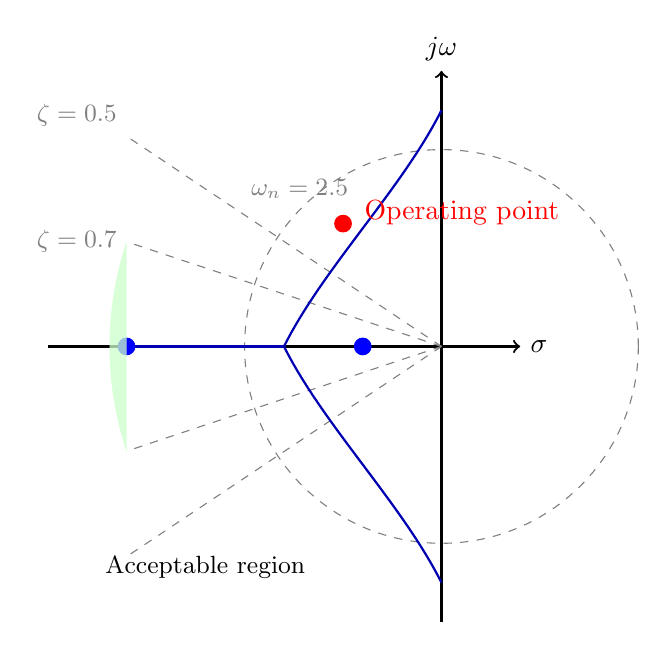
\begin{tikzpicture}[scale=1.0]
    % Axes
    \draw[->,thick] (-5,0) -- (1,0) node[right] {$\sigma$};
    \draw[->,thick] (0,-3.5) -- (0,3.5) node[above] {$j\omega$};

    % Constant damping ratio lines
    \draw[dashed,gray] (0,0) -- (-4,2.67) node[above left,font=\small] {$\zeta=0.5$};
    \draw[dashed,gray] (0,0) -- (-4,-2.67);
    \draw[dashed,gray] (0,0) -- (-4,1.33) node[left,font=\small] {$\zeta=0.7$};
    \draw[dashed,gray] (0,0) -- (-4,-1.33);

    % Constant natural frequency circle
    \draw[dashed,gray] (0,0) circle (2.5);
    \node[gray,font=\small] at (-1.8,2) {$\omega_n=2.5$};

    % Root locus (example)
    \draw[thick,blue!70!black] (-4,0) -- (-2,0);
    \draw[thick,blue!70!black] (-2,0) .. controls (-1.5,1) and (-0.5,2) .. (0,3);
    \draw[thick,blue!70!black] (-2,0) .. controls (-1.5,-1) and (-0.5,-2) .. (0,-3);

    % Poles
    \filldraw[blue] (-4,0) circle (3pt);
    \filldraw[blue] (-1,0) circle (3pt);

    % Operating point
    \filldraw[red] (-1.25,1.56) circle (3pt);
    \node[red,right] at (-1.1,1.7) {Operating point};

    % Region
    \fill[green!20,opacity=0.5] (-4,0) -- (-4,1.33) arc(161.6:198.4:4.22) -- cycle;
    \fill[green!20,opacity=0.5] (-4,0) -- (-4,-1.33) arc(-161.6:-198.4:4.22) -- cycle;

    \node[font=\small] at (-3,-2.8) {Acceptable region};
\end{tikzpicture}
\caption{Root locus with overlaid performance specifications: constant damping ratio lines and natural frequency circles define acceptable pole regions.}
\label{fig:gain_selection}
\end{figure}

\subsection{Parameter Sensitivity Analysis}

Beyond gain selection, root locus reveals how sensitive pole locations are to parameter changes. Regions where the locus passes nearly tangent to the imaginary axis indicate high sensitivity to gain variations---small changes in $K$ produce large changes in damping. Such systems require tight component tolerances or adaptive gain control.

\subsection{Educational Applications}

Root locus remains an essential pedagogical tool. Interactive software allowing students to modify pole-zero configurations and immediately observe the resulting locus changes builds intuition impossible to develop through equations alone. Many universities use root locus simulations as primary teaching tools in introductory control courses.

%=============================================================================
\section{Mathematical Foundation}
\label{sec:math_foundation}
%=============================================================================

We now develop the complete mathematical theory underlying the root locus method. Our goal is not merely to state the construction rules, but to derive each one rigorously so that the reader understands \textit{why} the method works.

\subsection{The Characteristic Equation}

Consider the standard negative feedback configuration shown in Figure~\ref{fig:feedback_block}.

\begin{figure}[H]
\centering
\begin{tikzpicture}[scale=1.0, auto, >=Stealth]
    % Summing junction
    \draw (0,0) circle (0.3);
    \draw (-0.15,0) -- (0.15,0);
    \draw (0,-0.15) -- (0,0.15);
    \node at (-0.5,0.3) {$+$};
    \node at (0.3,-0.5) {$-$};

    % Forward path
    \draw[->] (-2,0) -- (-0.3,0) node[midway,above] {$R(s)$};
    \draw[->] (0.3,0) -- (1.5,0) node[midway,above] {$E(s)$};
    \draw (1.5,-0.7) rectangle (3.5,0.7);
    \node at (2.5,0) {$KG(s)$};
    \draw[->] (3.5,0) -- (5.5,0) node[midway,above] {$Y(s)$};

    % Feedback path
    \draw (4.5,0) -- (4.5,-1.5);
    \draw (4.5,-1.5) -- (1,-1.5);
    \draw (1,-1.5) rectangle (2.5,-2.3);
    \node at (1.75,-1.9) {$H(s)$};
    \draw (1,-1.9) -- (0,-1.9);
    \draw[->] (0,-1.9) -- (0,-0.3);

    % Output tap
    \filldraw (4.5,0) circle (2pt);
\end{tikzpicture}
\caption{Standard negative feedback control system with forward path gain $K$, plant $G(s)$, and feedback transfer function $H(s)$.}
\label{fig:feedback_block}
\end{figure}

The closed-loop transfer function from $R(s)$ to $Y(s)$ is:
\begin{equation}
T(s) = \frac{KG(s)}{1 + KG(s)H(s)}
\label{eq:closed_loop_general}
\end{equation}

The closed-loop poles are the values of $s$ that make the denominator zero:
\begin{equation}
\boxed{1 + KG(s)H(s) = 0}
\label{eq:characteristic}
\end{equation}

This is the \textbf{characteristic equation} of the closed-loop system. Note that the closed-loop poles depend on the gain $K$, stability requires all roots of Eq.~\eqref{eq:characteristic} to have negative real parts, and transient response characteristics such as overshoot and settling time are determined by these pole locations.

\begin{definition}{Root Locus}{def:root_locus}
The \textbf{root locus} is the set of all points in the complex $s$-plane that satisfy the characteristic equation $1 + KG(s)H(s) = 0$ for some real, non-negative value of $K$. Equivalently, it is the locus of closed-loop poles as $K$ varies from $0$ to $\infty$.
\end{definition}

\subsection{The Loop Transfer Function}

Let the open-loop transfer function be expressed in factored form:
\begin{equation}
G(s)H(s) = \frac{(s-z_1)(s-z_2)\cdots(s-z_m)}{(s-p_1)(s-p_2)\cdots(s-p_n)}
\label{eq:GH_factored}
\end{equation}

where $z_1, z_2, \ldots, z_m$ are the open-loop zeros and $p_1, p_2, \ldots, p_n$ are the open-loop poles. We assume the system is proper, meaning $n \geq m$.

Rewriting the characteristic equation:
\begin{equation}
KG(s)H(s) = -1
\label{eq:KGH_minus1}
\end{equation}

Since $K > 0$ and $G(s)H(s)$ is a complex number for any $s$, this equation places constraints on both the magnitude and angle of $G(s)H(s)$.

\subsection{Magnitude and Angle Criteria}

Writing the complex number $-1$ in polar form: $-1 = 1 \angle 180°$. Equation~\eqref{eq:KGH_minus1} thus requires:

\begin{theorem}{Magnitude and Angle Criteria}{thm:criteria}
A point $s$ lies on the root locus if and only if it satisfies both criteria: the \textbf{Angle Criterion}, which requires $\angle G(s)H(s) = \pm 180°(2k+1)$ where $k = 0, 1, 2, \ldots$; and the \textbf{Magnitude Criterion}, which requires $|KG(s)H(s)| = 1$, giving $K = \frac{1}{|G(s)H(s)|}$.
\end{theorem}

\begin{proof}
From $KG(s)H(s) = -1$, we have:
\[
|KG(s)H(s)| = |-1| = 1
\]
and
\[
\angle KG(s)H(s) = \angle(-1) = 180° + n \cdot 360°, \quad n \in \mathbb{Z}
\]

Since $K > 0$, we have $\angle K = 0°$, giving:
\[
\angle G(s)H(s) = 180°(2k+1), \quad k = 0, 1, 2, \ldots
\]

The magnitude condition with $K > 0$ gives:
\[
K \cdot |G(s)H(s)| = 1 \implies K = \frac{1}{|G(s)H(s)|}
\]
\end{proof}

The crucial insight is that the angle criterion alone determines which points lie on the root locus. The magnitude criterion then determines the value of $K$ at each point. This separation makes graphical construction possible.

\subsection{Geometric Interpretation of the Angle Criterion}

For a point $s$ in the complex plane, we can write:
\begin{equation}
\angle G(s)H(s) = \sum_{i=1}^{m} \angle(s-z_i) - \sum_{j=1}^{n} \angle(s-p_j)
\label{eq:angle_sum}
\end{equation}

Each term $\angle(s-z_i)$ represents the angle of the vector drawn from zero $z_i$ to the point $s$. Similarly, $\angle(s-p_j)$ is the angle from pole $p_j$ to $s$.

\begin{figure}[H]
\centering
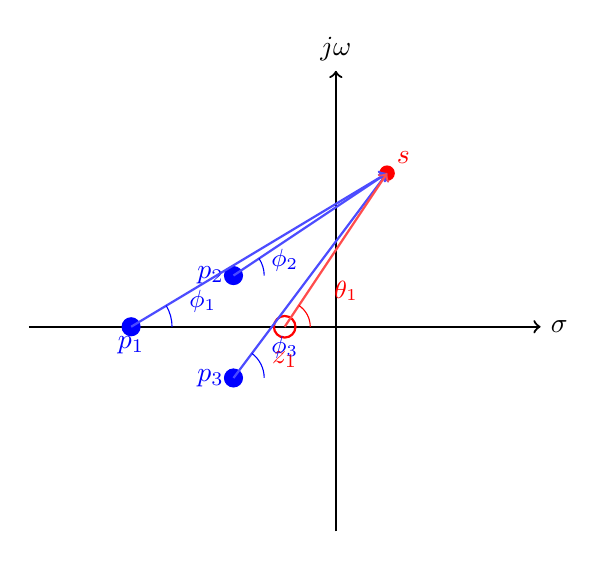
\begin{tikzpicture}[scale=1.3]
    % Axes
    \draw[->,thick] (-3,0) -- (2,0) node[right] {$\sigma$};
    \draw[->,thick] (0,-2) -- (0,2.5) node[above] {$j\omega$};

    % Point s
    \coordinate (S) at (0.5,1.5);
    \filldraw[red] (S) circle (2pt) node[above right] {$s$};

    % Poles
    \coordinate (P1) at (-2,0);
    \coordinate (P2) at (-1,0.5);
    \coordinate (P3) at (-1,-0.5);

    \filldraw[blue] (P1) circle (2.5pt);
    \node[blue,below] at (P1) {$p_1$};
    \filldraw[blue] (P2) circle (2.5pt);
    \node[blue,left] at (P2) {$p_2$};
    \filldraw[blue] (P3) circle (2.5pt);
    \node[blue,left] at (P3) {$p_3$};

    % Zero
    \coordinate (Z1) at (-0.5,0);
    \draw[red,thick] (Z1) circle (3pt);
    \node[red,below] at (-0.5,-0.15) {$z_1$};

    % Vectors from poles/zeros to s
    \draw[->,thick,blue!70] (P1) -- (S);
    \draw[->,thick,blue!70] (P2) -- (S);
    \draw[->,thick,blue!70] (P3) -- (S);
    \draw[->,thick,red!70] (Z1) -- (S);

    % Angles
    \draw[blue] (P1) ++(0.4,0) arc (0:31:0.4);
    \node[blue,font=\small] at (-1.3,0.25) {$\phi_1$};

    \draw[blue] (P2) ++(0.3,0) arc (0:34:0.3);
    \node[blue,font=\small] at (-0.5,0.65) {$\phi_2$};

    \draw[blue] (P3) ++(0.3,0) arc (0:53:0.3);
    \node[blue,font=\small] at (-0.5,-0.2) {$\phi_3$};

    \draw[red] (Z1) ++(0.25,0) arc (0:56.3:0.25);
    \node[red,font=\small] at (0.1,0.35) {$\theta_1$};
\end{tikzpicture}
\caption{Geometric interpretation: angles from poles ($\phi_i$) and zeros ($\theta_i$) to test point $s$. The angle criterion requires $\sum \theta_i - \sum \phi_i = \pm 180°(2k+1)$.}
\label{fig:angle_geometry}
\end{figure}

\subsection{Root Locus Construction Rules}

We now derive the eight fundamental rules for sketching root locus diagrams.

\subsubsection{Rule 1: Starting Points (K = 0)}

\begin{theorem}{Starting Points}{thm:start}
The root locus begins at the open-loop poles (when $K = 0$).
\end{theorem}

\begin{proof}
The characteristic equation is:
\[
1 + KG(s)H(s) = 0
\]

Rearranging:
\[
(s-p_1)(s-p_2)\cdots(s-p_n) + K(s-z_1)(s-z_2)\cdots(s-z_m) = 0
\]

As $K \to 0$, this approaches:
\[
(s-p_1)(s-p_2)\cdots(s-p_n) = 0
\]

whose roots are precisely the open-loop poles $p_1, p_2, \ldots, p_n$.
\end{proof}

\subsubsection{Rule 2: Ending Points (K → ∞)}

\begin{theorem}{Ending Points}{thm:end}
As $K \to \infty$, $m$ branches of the root locus approach the $m$ finite open-loop zeros. The remaining $n - m$ branches approach infinity along asymptotes.
\end{theorem}

\begin{proof}
Dividing the characteristic equation by $K$:
\[
\frac{1}{K} + G(s)H(s) = 0
\]

As $K \to \infty$, this becomes $G(s)H(s) = 0$, whose roots are the open-loop zeros $z_1, z_2, \ldots, z_m$.

Since the characteristic polynomial has degree $n$, there are always $n$ roots. With $m$ approaching finite zeros, the remaining $n - m$ roots must approach infinity.
\end{proof}

\subsubsection{Rule 3: Number of Branches}

\begin{theorem}{Number of Branches}{thm:branches}
The root locus has $n$ branches, where $n$ is the number of open-loop poles.
\end{theorem}

\begin{proof}
The characteristic equation $1 + KG(s)H(s) = 0$, when cleared of fractions, yields a polynomial of degree $n$ in $s$. By the fundamental theorem of algebra, this polynomial has exactly $n$ roots (counting multiplicity). Each root traces a continuous path as $K$ varies, forming one branch of the locus.
\end{proof}

\subsubsection{Rule 4: Symmetry}

\begin{theorem}{Real Axis Symmetry}{thm:symmetry}
The root locus is symmetric about the real axis.
\end{theorem}

\begin{proof}
The characteristic polynomial has real coefficients (since $G(s)H(s)$ represents a physical system with real parameters and $K$ is real). Complex roots of polynomials with real coefficients occur in conjugate pairs. Therefore, if $s_0 = \sigma + j\omega$ is on the root locus, so is $\bar{s}_0 = \sigma - j\omega$.
\end{proof}

\subsubsection{Rule 5: Real Axis Segments}

\begin{theorem}{Real Axis Segments}{thm:real_axis}
A point on the real axis belongs to the root locus if and only if it lies to the left of an odd total number of real poles and zeros.
\end{theorem}

\begin{proof}
Consider a test point $s = \sigma$ on the real axis (where $\sigma$ is real). For the angle criterion:
\[
\angle G(\sigma)H(\sigma) = \sum \angle(\sigma - z_i) - \sum \angle(\sigma - p_j)
\]

For a complex conjugate pair of poles $p = \alpha \pm j\beta$:
\[
\angle(\sigma - p) + \angle(\sigma - \bar{p}) = \theta + (-\theta) = 0
\]

since the angles from conjugate poles to any real point are equal and opposite. Thus, complex pole-zero pairs contribute zero net angle.

For a \textbf{real} pole or zero, the angle contribution depends on the test point's position: if $\sigma$ is to the \textbf{right} of the singularity, the angle contribution is $0°$, whereas if $\sigma$ is to the \textbf{left} of the singularity, the angle contribution is $\pm 180°$.

\begin{figure}[H]
\centering
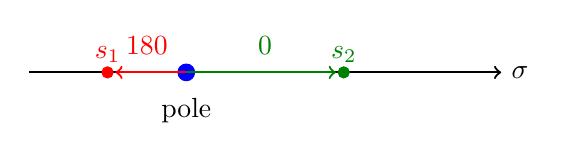
\begin{tikzpicture}[scale=1.0]
    % Axis
    \draw[->,thick] (-4,0) -- (2,0) node[right] {$\sigma$};

    % Real pole
    \filldraw[blue] (-2,0) circle (3pt);
    \node[below] at (-2,-0.2) {pole};

    % Test points
    \filldraw[red] (-3,0) circle (2pt) node[above] {$s_1$};
    \filldraw[green!50!black] (0,0) circle (2pt) node[above] {$s_2$};

    % Vectors
    \draw[->,thick,red] (-2,0) -- (-2.9,0);
    \node[red,above] at (-2.5,0.1) {$180°$};

    \draw[->,thick,green!50!black] (-2,0) -- (-0.1,0);
    \node[green!50!black,above] at (-1,0.1) {$0°$};
\end{tikzpicture}
\caption{Angle contribution from a real pole: $180°$ for points to its left, $0°$ for points to its right.}
\label{fig:real_axis_angle}
\end{figure}

Each real pole or zero to the right of the test point contributes $0°$. Each real pole or zero to the left contributes $\pm 180°$ (positive for zeros, negative for poles, but the absolute values are what matter for the criterion).

For the angle criterion $\angle G(s)H(s) = \pm 180°(2k+1)$ to be satisfied, the total angle must be an odd multiple of $180°$. This occurs if and only if there is an odd number of real poles and zeros to the right of the test point.
\end{proof}

\begin{figure}[H]
\centering
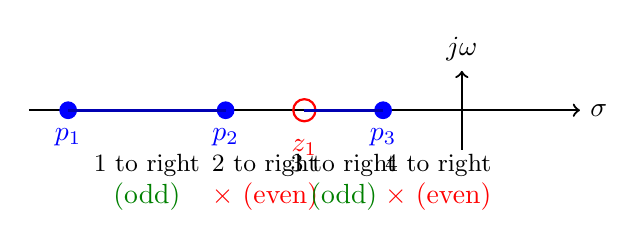
\begin{tikzpicture}[scale=1.0]
    % Axes
    \draw[->,thick] (-5.5,0) -- (1.5,0) node[right] {$\sigma$};
    \draw[->,thick] (0,-0.5) -- (0,0.5) node[above] {$j\omega$};

    % Poles
    \filldraw[blue] (-5,0) circle (3pt) node[below=3pt] {$p_1$};
    \filldraw[blue] (-3,0) circle (3pt) node[below=3pt] {$p_2$};
    \filldraw[blue] (-1,0) circle (3pt) node[below=3pt] {$p_3$};

    % Zero
    \draw[red,thick] (-2,0) circle (4pt);
    \node[red,below] at (-2,-0.25) {$z_1$};

    % Root locus segments on real axis
    \draw[very thick,blue!70!black] (-5,0) -- (-3,0);
    \draw[very thick,blue!70!black] (-2,0) -- (-1,0);

    % Counting labels
    \node[font=\small] at (-4,-0.7) {1 to right};
    \node[font=\small] at (-2.5,-0.7) {2 to right};
    \node[font=\small] at (-1.5,-0.7) {3 to right};
    \node[font=\small] at (-0.3,-0.7) {4 to right};

    % Checkmarks
    \node[green!50!black] at (-4,-1.1) {\checkmark (odd)};
    \node[red] at (-2.5,-1.1) {$\times$ (even)};
    \node[green!50!black] at (-1.5,-1.1) {\checkmark (odd)};
    \node[red] at (-0.3,-1.1) {$\times$ (even)};
\end{tikzpicture}
\caption{Real axis segments (thick lines) occur where an odd number of poles plus zeros lie to the right.}
\label{fig:real_axis_rule}
\end{figure}

\subsubsection{Rule 6: Asymptotes}

\begin{theorem}{Asymptotes}{thm:asymptotes}
The $n - m$ branches approaching infinity do so along asymptotes that have angles $\theta_a = \frac{(2k+1) \cdot 180°}{n-m}$ for $k = 0, 1, \ldots, n-m-1$, and intersect the real axis at the centroid $\sigma_a = \frac{\sum_{i=1}^{n} p_i - \sum_{j=1}^{m} z_j}{n-m}$.
\end{theorem}

\begin{proof}
\textbf{(Asymptote angles):} For large $|s|$, all poles and zeros appear clustered near the origin when viewed from $s$. The transfer function behaves as:
\[
G(s)H(s) \approx \frac{s^m}{s^n} = \frac{1}{s^{n-m}}
\]

The angle criterion becomes:
\[
\angle\left(\frac{1}{s^{n-m}}\right) = -(n-m)\angle s = (2k+1) \cdot 180°
\]

Therefore:
\[
\angle s = \frac{(2k+1) \cdot 180°}{n-m}
\]

\textbf{(Centroid):} The asymptotes emanate from a common point $\sigma_a$ on the real axis. To find this point, we analyze the characteristic equation for large $s$ more carefully.

Let $s = \sigma_a + re^{j\theta}$ where $r$ is large. The characteristic equation:
\[
1 + K\frac{\prod(s-z_j)}{\prod(s-p_i)} = 0
\]

For large $r$, using the approximation $\ln(1+x) \approx x$ for small $x$:
\[
\sum_{j=1}^{m} \ln(s-z_j) - \sum_{i=1}^{n} \ln(s-p_i) = \ln(-1/K)
\]

Expanding $\ln(s-a) = \ln s + \ln(1 - a/s) \approx \ln s - a/s$ for $|s| >> |a|$:
\[
m\ln s - \sum z_j/s - n\ln s + \sum p_i/s = \ln(-1/K)
\]

For the asymptotes to pass through $\sigma_a$, the $O(1/s)$ terms must cancel when $s$ is on an asymptote:
\[
\frac{\sum p_i - \sum z_j}{s} = 0 \text{ relative to the asymptote center}
\]

This gives:
\[
\sigma_a = \frac{\sum_{i=1}^{n} p_i - \sum_{j=1}^{m} z_j}{n - m}
\]
\end{proof}

\begin{figure}[H]
\centering
\begin{tikzpicture}[scale=0.9]
    % Axes
    \draw[->,thick] (-4,0) -- (3,0) node[right] {$\sigma$};
    \draw[->,thick] (0,-3.5) -- (0,3.5) node[above] {$j\omega$};

    % Example: 3 poles, 1 zero => 2 asymptotes at ±90°
    % Poles at -1, -2, -3; Zero at -0.5
    % Centroid = (-1-2-3 - (-0.5))/2 = -5.5/2 = -2.75

    \coordinate (centroid) at (-2.75,0);
    \filldraw[green!50!black] (centroid) circle (2pt);
    \node[below] at (centroid) {$\sigma_a$};

    % Asymptotes
    \draw[dashed,thick,purple] (centroid) -- ++(0,3.2);
    \draw[dashed,thick,purple] (centroid) -- ++(0,-3.2);

    % Poles
    \filldraw[blue] (-1,0) circle (3pt);
    \filldraw[blue] (-2,0) circle (3pt);
    \filldraw[blue] (-3,0) circle (3pt);

    % Zero
    \draw[red,thick] (-0.5,0) circle (4pt);

    % Angle labels
    \draw[->] (-2.75,1.5) arc (90:0:0.5);
    \node at (-1.9,1.3) {$90°$};

    \draw[->] (-2.75,-1.5) arc (-90:0:0.5);
    \node at (-1.9,-1.3) {$-90°$};

    % Title
    \node at (-0.5,-4) {$n=3$, $m=1$: asymptotes at $\pm 90°$};
\end{tikzpicture}
\hspace{1cm}
\begin{tikzpicture}[scale=0.9]
    % Axes
    \draw[->,thick] (-4,0) -- (3,0) node[right] {$\sigma$};
    \draw[->,thick] (0,-3.5) -- (0,3.5) node[above] {$j\omega$};

    % Example: 3 poles, 0 zeros => 3 asymptotes at 60°, 180°, -60°
    % Centroid = (-1-2-3)/3 = -2

    \coordinate (centroid) at (-2,0);
    \filldraw[green!50!black] (centroid) circle (2pt);
    \node[below right] at (centroid) {$\sigma_a$};

    % Asymptotes
    \draw[dashed,thick,purple] (centroid) -- ++(60:3);
    \draw[dashed,thick,purple] (centroid) -- ++(180:2);
    \draw[dashed,thick,purple] (centroid) -- ++(-60:3);

    % Poles
    \filldraw[blue] (-1,0) circle (3pt);
    \filldraw[blue] (-2,0) circle (3pt);
    \filldraw[blue] (-3,0) circle (3pt);

    % Angle labels
    \draw[->] (-1.3,0) arc (0:60:0.7);
    \node at (-0.8,0.6) {$60°$};

    % Title
    \node at (-0.5,-4) {$n=3$, $m=0$: asymptotes at $60°, 180°, -60°$};
\end{tikzpicture}
\caption{Asymptote construction examples showing centroid location and asymptote angles.}
\label{fig:asymptotes}
\end{figure}

\subsubsection{Rule 7: Breakaway and Break-in Points}

\begin{theorem}{Breakaway and Break-in Points}{thm:breakaway}
Breakaway points (where branches leave the real axis) and break-in points (where branches arrive at the real axis) occur at values of $s$ satisfying:
\[
\frac{dK}{ds} = 0
\]
where $K$ is expressed as a function of $s$ from the magnitude condition.
\end{theorem}

\begin{proof}
On the real axis portion of the root locus, the gain $K$ at any point $s = \sigma$ is:
\[
K = \frac{1}{|G(\sigma)H(\sigma)|} = \left|\frac{\prod(\sigma - p_i)}{\prod(\sigma - z_j)}\right|
\]

At a breakaway point, two branches of the locus merge and leave the real axis. Since each branch corresponds to a different root of the characteristic equation, at the breakaway point these roots are equal---a repeated root occurs.

For a polynomial equation to have a repeated root, the root must also be a root of the derivative. Equivalently, $K(\sigma)$ must have a local maximum or minimum at the breakaway point.

\textbf{Alternative derivation:} From $1 + KG(s)H(s) = 0$:
\[
K = -\frac{1}{G(s)H(s)}
\]

Differentiating:
\[
\frac{dK}{ds} = \frac{d}{ds}\left[-\frac{1}{G(s)H(s)}\right] = \frac{1}{[G(s)H(s)]^2}\frac{d[G(s)H(s)]}{ds}
\]

Setting $\frac{dK}{ds} = 0$ and noting $G(s)H(s) \neq 0$ at breakaway points:
\[
\frac{d[G(s)H(s)]}{ds} = 0
\]

This can be written more conveniently as:
\[
\sum_{j=1}^{m} \frac{1}{s-z_j} = \sum_{i=1}^{n} \frac{1}{s-p_i}
\]
\end{proof}

\begin{examplebox}[Finding Breakaway Points]
\label{ex:breakaway}
For $G(s)H(s) = \frac{1}{s(s+4)}$, find the breakaway point.

\textbf{Solution:} From the magnitude condition:
\[
K = |s(s+4)| = |s^2 + 4s|
\]

On the real axis between $s = -4$ and $s = 0$ (the root locus segment):
\[
K = \sigma(\sigma + 4) = \sigma^2 + 4\sigma
\]

Taking the derivative and setting to zero:
\[
\frac{dK}{d\sigma} = 2\sigma + 4 = 0 \implies \sigma = -2
\]

The breakaway point is at $s = -2$, where $K = (-2)(-2+4) = 4$.
\end{examplebox}

\subsubsection{Rule 8: Imaginary Axis Crossings}

\begin{theorem}{Imaginary Axis Crossings}{thm:jw_crossing}
The values of $K$ and $\omega$ where the root locus crosses the imaginary axis can be found by either substituting $s = j\omega$ into the characteristic equation and solving for $K$ and $\omega$, or by using the Routh-Hurwitz criterion to find the value of $K$ that produces a row of zeros.
\end{theorem}

\begin{proof}
If $s = j\omega$ is a root of the characteristic equation, then it must satisfy:
\[
1 + KG(j\omega)H(j\omega) = 0
\]

Separating into real and imaginary parts gives two equations in two unknowns ($K$ and $\omega$), which can be solved simultaneously.

Alternatively, the Routh array for the characteristic polynomial will have a row of zeros when the polynomial has pure imaginary roots. The gain $K$ that causes this can be found from the Routh stability criterion, and the crossing frequency from the auxiliary polynomial.
\end{proof}

\begin{examplebox}[Finding Imaginary Axis Crossing]
\label{ex:jw_cross}
For the system with $G(s)H(s) = \frac{K}{s(s+1)(s+2)}$, find where the root locus crosses the imaginary axis.

\textbf{Solution:} The characteristic equation is:
\[
s^3 + 3s^2 + 2s + K = 0
\]

Forming the Routh array:
\[
\begin{array}{c|cc}
s^3 & 1 & 2 \\
s^2 & 3 & K \\
s^1 & \frac{6-K}{3} & 0 \\
s^0 & K &
\end{array}
\]

For marginal stability (imaginary axis crossing), the $s^1$ row must be zero:
\[
\frac{6-K}{3} = 0 \implies K = 6
\]

The auxiliary polynomial from the $s^2$ row is:
\[
3s^2 + K = 3s^2 + 6 = 0 \implies s = \pm j\sqrt{2}
\]

The root locus crosses the imaginary axis at $s = \pm j\sqrt{2}$ when $K = 6$.
\end{examplebox}

\subsection{Gain Determination from Root Locus}

Once a root locus is sketched, the gain $K$ at any point can be found from the magnitude criterion:
\begin{equation}
K = \frac{\prod_{i=1}^{n} |s - p_i|}{\prod_{j=1}^{m} |s - z_j|} = \frac{\text{Product of distances from poles}}{\text{Product of distances from zeros}}
\label{eq:gain_formula}
\end{equation}

This geometric interpretation allows gain determination directly from the plot by measuring distances.

\begin{figure}[H]
\centering
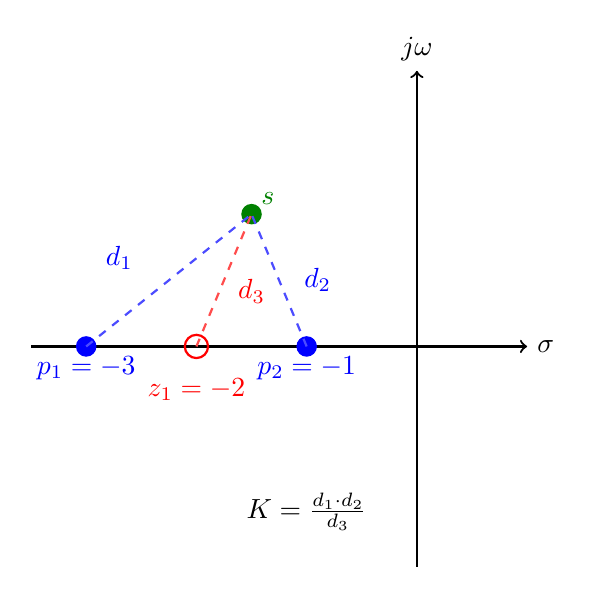
\begin{tikzpicture}[scale=1.4]
    % Axes
    \draw[->,thick] (-3.5,0) -- (1,0) node[right] {$\sigma$};
    \draw[->,thick] (0,-2) -- (0,2.5) node[above] {$j\omega$};

    % Poles
    \filldraw[blue] (-3,0) circle (2.5pt) node[below] {$p_1=-3$};
    \filldraw[blue] (-1,0) circle (2.5pt) node[below] {$p_2=-1$};

    % Zero
    \draw[red,thick] (-2,0) circle (3pt);
    \node[red,below] at (-2,-0.2) {$z_1=-2$};

    % Test point on locus
    \coordinate (S) at (-1.5,1.2);
    \filldraw[green!50!black] (S) circle (2.5pt) node[above right] {$s$};

    % Distance vectors
    \draw[thick,blue!70,dashed] (-3,0) -- (S);
    \draw[thick,blue!70,dashed] (-1,0) -- (S);
    \draw[thick,red!70,dashed] (-2,0) -- (S);

    % Distance labels
    \node[blue] at (-2.7,0.8) {$d_1$};
    \node[blue] at (-0.9,0.6) {$d_2$};
    \node[red] at (-1.5,0.5) {$d_3$};

    % Formula
    \node at (-1,-1.5) {$K = \frac{d_1 \cdot d_2}{d_3}$};
\end{tikzpicture}
\caption{Gain calculation from the root locus: $K$ equals the product of distances from the test point to all poles, divided by the product of distances to all zeros.}
\label{fig:gain_calculation}
\end{figure}

%=============================================================================
\section{Practical Experiments}
\label{sec:experiments}
%=============================================================================

Understanding root locus deeply requires hands-on exploration. This section presents both simulation-based and hardware-based experiments that reinforce the theoretical concepts.

\subsection{Interactive Root Locus Visualization}

The following algorithm describes an interactive root locus visualization with a slider to vary gain $K$. The display simultaneously shows the pole locations and the corresponding step response.

\begin{algorithm}
\caption{Interactive Root Locus Visualization}
\begin{algorithmic}[1]
\State Define open-loop transfer function $G(s) = \frac{1}{s(s+1)(s+3)}$
\State Initialize gain $K \gets K_{\text{init}}$
\State Create side-by-side plot panels for root locus and step response
\State \textbf{function} ComputeClosedLoopPoles($K$):
\State \hspace{1em} Form characteristic polynomial: $s^3 + 4s^2 + 3s + K = 0$
\State \hspace{1em} \Return roots of characteristic polynomial
\State \textbf{function} ComputeStepResponse($K$, $t$):
\State \hspace{1em} Form closed-loop transfer function $T(s) = \frac{K}{s^3 + 4s^2 + 3s + K}$
\State \hspace{1em} \Return step response evaluated at time vector $t$
\For{$K$ from $K_{\min}$ to $K_{\max}$}
\State Compute poles for this $K$ and store trajectory
\EndFor
\State Plot complete root locus trajectories
\State Mark open-loop pole locations
\State Create interactive slider for gain $K$
\While{user adjusts slider}
\State $K \gets$ slider value
\State poles $\gets$ \Call{ComputeClosedLoopPoles}{$K$}
\State Update pole marker positions on root locus plot
\State $y \gets$ \Call{ComputeStepResponse}{$K$, $t$}
\State Update step response plot
\If{any pole has positive real part}
\State Display ``UNSTABLE'' warning
\EndIf
\State Refresh display
\EndWhile
\end{algorithmic}
\end{algorithm}

\subsection{Alternative Implementation}

For those using other computational environments, Algorithm 2 describes the same interactive root locus visualization approach. The key steps involve defining the open-loop system, computing the root locus trajectories for a range of gain values, and creating an interactive interface that updates both the pole locations and step response as the user adjusts the gain.

\subsection{Physical Experiment: DC Motor Speed Control}

This experiment demonstrates root locus concepts using a real DC motor system.

The required equipment includes a DC motor with tachometer feedback, an adjustable gain amplifier (or microcontroller with DAC), an oscilloscope for response measurement, and a function generator for providing step inputs.

\textbf{Procedure:}

The experiment proceeds in four phases. First, perform \textbf{system identification} by applying a step voltage to the motor and recording the open-loop response, then fit a first or second-order transfer function model to the measured data. Second, construct the \textbf{theoretical root locus} using the identified model, calculating and sketching the expected root locus to predict the gain $K_{crit}$ at which instability occurs, the oscillation frequency at marginal stability, and the gain for optimal damping (e.g., $\zeta = 0.7$). Third, conduct \textbf{experimental verification} by closing the feedback loop with low gain and recording the step response, then gradually increasing the gain while recording step responses at each setting, noting the onset of oscillations and eventual instability, and measuring the oscillation frequency at marginal stability. Finally, perform \textbf{data analysis} by comparing the experimental $K_{crit}$ with the theoretical prediction, comparing the measured oscillation frequency with the predicted $j\omega$-axis crossing, and plotting the experimental damping ratio versus gain to compare with root locus predictions.

\textbf{Expected Results:}

For a typical DC motor with transfer function $G(s) = \frac{K_m}{\tau s + 1}$ in a unity feedback configuration, the root locus is a simple horizontal line from $-1/\tau$ toward $-\infty$. The system is always stable for positive $K$.

Adding a second pole (representing electrical dynamics or load inertia) creates the possibility of instability. For $G(s) = \frac{K_m}{(s+a)(s+b)}$, the root locus will show breakaway from the real axis and eventual crossing into the right half-plane.

\begin{figure}[H]
\centering
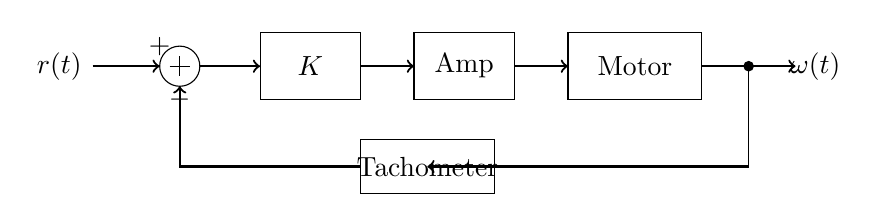
\begin{tikzpicture}[scale=0.85]
    % Block diagram of motor control experiment

    % Input
    \node at (-4,0) {$r(t)$};
    \draw[->,thick] (-3.5,0) -- (-2.5,0);

    % Summing junction
    \draw (-2.2,0) circle (0.3);
    \draw (-2.35,0) -- (-2.05,0);
    \draw (-2.2,0.15) -- (-2.2,-0.15);
    \node at (-2.5,0.3) {$+$};
    \node at (-2.2,-0.5) {$-$};

    % Controller
    \draw[->,thick] (-1.9,0) -- (-1,0);
    \draw (-1,-0.5) rectangle (0.5,0.5);
    \node at (-0.25,0) {$K$};

    % Amplifier
    \draw[->,thick] (0.5,0) -- (1.3,0);
    \draw (1.3,-0.5) rectangle (2.8,0.5);
    \node at (2.05,0) {Amp};

    % Motor
    \draw[->,thick] (2.8,0) -- (3.6,0);
    \draw (3.6,-0.5) rectangle (5.6,0.5);
    \node at (4.6,0) {Motor};

    % Output
    \draw[->,thick] (5.6,0) -- (7,0);
    \node at (7.3,0) {$\omega(t)$};

    % Tachometer feedback
    \draw (6.3,0) -- (6.3,-1.5);
    \draw[->,thick] (6.3,-1.5) -- (1.5,-1.5);
    \draw (0.5,-1.9) rectangle (2.5,-1.1);
    \node at (1.5,-1.5) {Tachometer};
    \draw[->,thick] (0.5,-1.5) -- (-2.2,-1.5) -- (-2.2,-0.3);

    \filldraw (6.3,0) circle (2pt);
\end{tikzpicture}
\caption{Block diagram of DC motor speed control experiment setup.}
\label{fig:motor_experiment}
\end{figure}

%=============================================================================
\section{Worked Examples}
\label{sec:examples}
%=============================================================================

\begin{example}{Basic Root Locus Sketch}{ex:basic}
Sketch the root locus for the system with open-loop transfer function:
\[
G(s)H(s) = \frac{K}{s(s+2)(s+4)}
\]

\textbf{Solution:}

\textit{Step 1: Identify poles and zeros.} The system has open-loop poles at $p_1 = 0$, $p_2 = -2$, and $p_3 = -4$, with no open-loop zeros ($m = 0$). Therefore, there are $n = 3$ branches.

\textit{Step 2: Real axis segments.} Count poles plus zeros to the right of each region. Right of $s = 0$ there are 0 poles/zeros (even, not on locus). Between $s = 0$ and $s = -2$ there is 1 pole (odd, \textbf{on locus}). Between $s = -2$ and $s = -4$ there are 2 poles (even, not on locus). Left of $s = -4$ there are 3 poles (odd, \textbf{on locus}).

\textit{Step 3: Asymptotes}

With $n - m = 3$ branches going to infinity:
\begin{align*}
\theta_a &= \frac{(2k+1) \cdot 180°}{3} = 60°, 180°, -60° \quad (k = 0, 1, 2)\\
\sigma_a &= \frac{(0 + (-2) + (-4)) - 0}{3} = -2
\end{align*}

\textit{Step 4: Breakaway point}

From $K = s(s+2)(s+4) = s^3 + 6s^2 + 8s$:
\[
\frac{dK}{ds} = 3s^2 + 12s + 8 = 0
\]

Using the quadratic formula:
\[
s = \frac{-12 \pm \sqrt{144 - 96}}{6} = \frac{-12 \pm 6.93}{6}
\]

This gives $s = -0.845$ or $s = -3.15$.

Only $s = -0.845$ lies on the root locus (between 0 and $-2$), so the breakaway point is at $s = -0.845$.

\textit{Step 5: Imaginary axis crossing}

Using Routh-Hurwitz on $s^3 + 6s^2 + 8s + K = 0$:
\[
\begin{array}{c|cc}
s^3 & 1 & 8 \\
s^2 & 6 & K \\
s^1 & \frac{48-K}{6} & 0 \\
s^0 & K &
\end{array}
\]

For marginal stability: $\frac{48-K}{6} = 0 \implies K = 48$

The crossing frequency from the auxiliary equation $6s^2 + 48 = 0$:
\[
s = \pm j\sqrt{8} = \pm j2\sqrt{2} \approx \pm j2.83
\]

\begin{figure}[H]
\centering
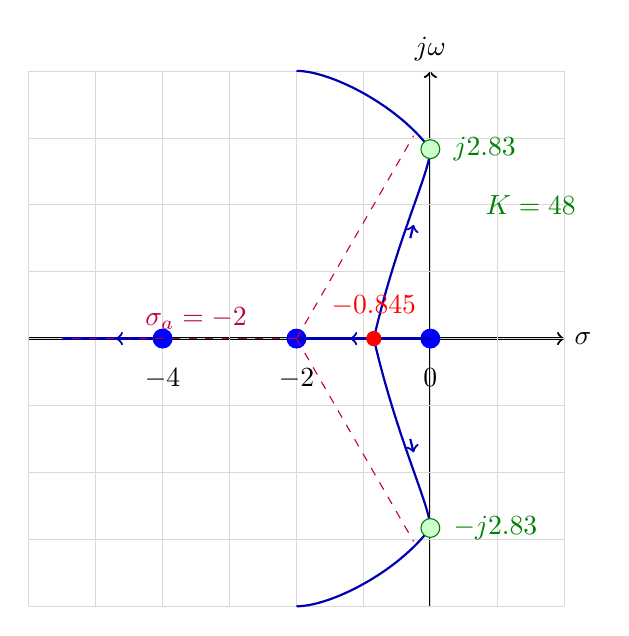
\begin{tikzpicture}[scale=0.85]
    % Axes
    \draw[->,thick] (-6,0) -- (2,0) node[right] {$\sigma$};
    \draw[->,thick] (0,-4) -- (0,4) node[above] {$j\omega$};

    % Grid
    \draw[gray!30,very thin] (-6,-4) grid (2,4);

    % Open-loop poles
    \filldraw[blue] (0,0) circle (4pt);
    \filldraw[blue] (-2,0) circle (4pt);
    \filldraw[blue] (-4,0) circle (4pt);
    \node[below] at (0,-0.3) {$0$};
    \node[below] at (-2,-0.3) {$-2$};
    \node[below] at (-4,-0.3) {$-4$};

    % Real axis segments
    \draw[very thick,blue!70!black] (0,0) -- (-2,0);
    \draw[very thick,blue!70!black] (-4,0) -- (-5.5,0);

    % Asymptotes
    \draw[dashed,purple] (-2,0) -- ++(60:3.5);
    \draw[dashed,purple] (-2,0) -- ++(180:3.5);
    \draw[dashed,purple] (-2,0) -- ++(-60:3.5);
    \node[purple] at (-3.5,0.3) {$\sigma_a = -2$};

    % Root locus branches
    \draw[thick,blue!70!black] (-0.845,0) .. controls (-0.5,1.5) and (0,2.5) .. (0,2.83);
    \draw[thick,blue!70!black] (-0.845,0) .. controls (-0.5,-1.5) and (0,-2.5) .. (0,-2.83);
    \draw[thick,blue!70!black] (0,2.83) .. controls (-0.5,3.5) and (-1.5,4) .. (-2,4);
    \draw[thick,blue!70!black] (0,-2.83) .. controls (-0.5,-3.5) and (-1.5,-4) .. (-2,-4);

    % Breakaway point
    \filldraw[red] (-0.845,0) circle (3pt);
    \node[red,above] at (-0.845,0.2) {$-0.845$};

    % jw crossing
    \draw[green!50!black,fill=green!20] (0,2.83) circle (4pt);
    \draw[green!50!black,fill=green!20] (0,-2.83) circle (4pt);
    \node[right,green!50!black] at (0.2,2.83) {$j2.83$};
    \node[right,green!50!black] at (0.2,-2.83) {$-j2.83$};
    \node[green!50!black] at (1.5,2) {$K=48$};

    % Arrows showing direction
    \draw[->,thick,blue!70!black] (-1,0) -- (-1.2,0);
    \draw[->,thick,blue!70!black] (-4.5,0) -- (-4.7,0);
    \draw[->,thick,blue!70!black] (-0.3,1.5) -- (-0.25,1.7);
    \draw[->,thick,blue!70!black] (-0.3,-1.5) -- (-0.25,-1.7);
\end{tikzpicture}
\caption{Complete root locus for Example 12.1: $G(s)H(s) = K/[s(s+2)(s+4)]$.}
\label{fig:example1_locus}
\end{figure}
\end{example}

\begin{example}{Root Locus with Zero}{ex:with_zero}
Sketch the root locus for:
\[
G(s)H(s) = \frac{K(s+3)}{s(s+1)(s+5)}
\]

\textbf{Solution:}

\textit{Step 1: Identify poles and zeros.} The system has open-loop poles at $p_1 = 0$, $p_2 = -1$, and $p_3 = -5$, with one open-loop zero at $z_1 = -3$. Thus $n = 3$, $m = 1$, and $n - m = 2$ branches go to infinity.

\textit{Step 2: Real axis segments.} Counting poles and zeros to the right of each region: for $s > 0$ there are 0 singularities (not on locus); for $-1 < s < 0$ there is 1 pole at 0 (\textbf{on locus}); for $-3 < s < -1$ there are 2 singularities (not on locus); for $-5 < s < -3$ there are 3 singularities including the zero at $-3$ (\textbf{on locus}); and for $s < -5$ there are 4 singularities (not on locus).

\textit{Step 3: Asymptotes}
\begin{align*}
\theta_a &= \frac{(2k+1) \cdot 180°}{2} = 90°, -90° \quad (k = 0, 1)\\
\sigma_a &= \frac{(0 - 1 - 5) - (-3)}{2} = \frac{-3}{2} = -1.5
\end{align*}

\textit{Step 4: Breakaway points}

From $K = \frac{s(s+1)(s+5)}{s+3}$:

Using the formula $\sum \frac{1}{s-p_i} = \sum \frac{1}{s-z_j}$:
\[
\frac{1}{s} + \frac{1}{s+1} + \frac{1}{s+5} = \frac{1}{s+3}
\]

Solving this equation (after algebraic manipulation) yields breakaway points at approximately $s = -0.473$ and a break-in point at $s = -3.52$.

\textit{Step 5: Ending points.} As $K \to \infty$, one branch ends at the zero $s = -3$, while the remaining two branches go to infinity along the asymptotes at $\pm 90°$.

\begin{figure}[H]
\centering
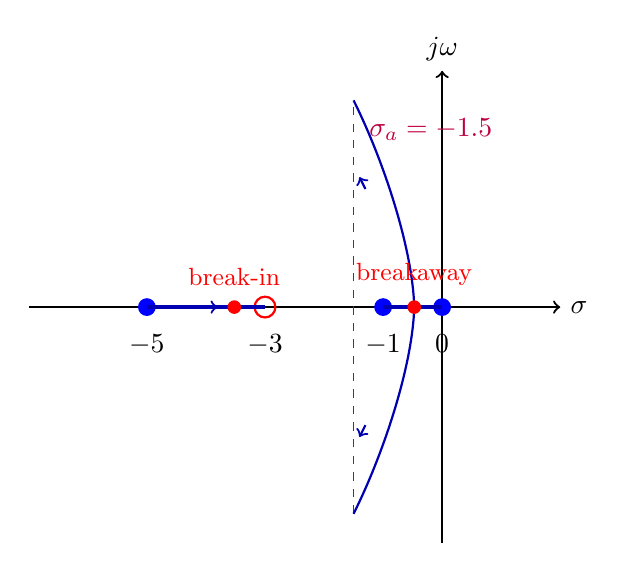
\begin{tikzpicture}[scale=0.75]
    % Axes
    \draw[->,thick] (-7,0) -- (2,0) node[right] {$\sigma$};
    \draw[->,thick] (0,-4) -- (0,4) node[above] {$j\omega$};

    % Poles
    \filldraw[blue] (0,0) circle (4pt);
    \filldraw[blue] (-1,0) circle (4pt);
    \filldraw[blue] (-5,0) circle (4pt);

    % Zero
    \draw[red,thick] (-3,0) circle (5pt);

    % Labels
    \node[below] at (0,-0.3) {$0$};
    \node[below] at (-1,-0.3) {$-1$};
    \node[below] at (-3,-0.3) {$-3$};
    \node[below] at (-5,-0.3) {$-5$};

    % Real axis segments
    \draw[very thick,blue!70!black] (0,0) -- (-1,0);
    \draw[very thick,blue!70!black] (-3,0) -- (-5,0);

    % Asymptotes
    \draw[dashed,purple] (-1.5,-3.5) -- (-1.5,3.5);
    \node[purple,right] at (-1.4,3) {$\sigma_a = -1.5$};

    % Root locus branches
    % Branch from 0 to breakaway then up
    \draw[thick,blue!70!black] (-0.473,0) .. controls (-0.5,1) and (-1,2.5) .. (-1.5,3.5);
    \draw[thick,blue!70!black] (-0.473,0) .. controls (-0.5,-1) and (-1,-2.5) .. (-1.5,-3.5);

    % Branch from -1 to breakaway
    \draw[thick,blue!70!black] (0,0) -- (-0.473,0);
    \draw[thick,blue!70!black] (-1,0) -- (-0.473,0);

    % Branch from -5 to break-in then to zero
    \draw[thick,blue!70!black] (-5,0) -- (-3.52,0);
    \draw[thick,blue!70!black] (-3.52,0) -- (-3,0);

    % Breakaway and break-in points
    \filldraw[red] (-0.473,0) circle (3pt);
    \filldraw[red] (-3.52,0) circle (3pt);
    \node[red,above] at (-0.473,0.2) {\small breakaway};
    \node[red,above] at (-3.52,0.2) {\small break-in};

    % Arrows
    \draw[->,thick,blue!70!black] (-1.3,2) -- (-1.4,2.2);
    \draw[->,thick,blue!70!black] (-1.3,-2) -- (-1.4,-2.2);
    \draw[->,thick,blue!70!black] (-4,0) -- (-3.8,0);
\end{tikzpicture}
\caption{Root locus for Example 12.2 showing breakaway point, break-in point, and asymptotes.}
\label{fig:example2_locus}
\end{figure}
\end{example}

\begin{example}{Asymptote Calculation}{ex:asymptotes}
For the system $G(s) = \frac{K}{(s+1)(s+2)(s+3)(s+4)}$, calculate the asymptotes.

\textbf{Solution:}

Poles: $-1, -2, -3, -4$ (n = 4)
Zeros: none (m = 0)
Branches to infinity: $n - m = 4$

\textbf{Asymptote angles:}
\[
\theta_a = \frac{(2k+1) \cdot 180°}{4} \text{ for } k = 0, 1, 2, 3
\]

\begin{align*}
k = 0: \quad \theta_a &= \frac{180°}{4} = 45° \\
k = 1: \quad \theta_a &= \frac{3 \cdot 180°}{4} = 135° \\
k = 2: \quad \theta_a &= \frac{5 \cdot 180°}{4} = 225° = -135° \\
k = 3: \quad \theta_a &= \frac{7 \cdot 180°}{4} = 315° = -45°
\end{align*}

\textbf{Centroid:}
\[
\sigma_a = \frac{(-1) + (-2) + (-3) + (-4)}{4} = \frac{-10}{4} = -2.5
\]

The four asymptotes emanate from $\sigma = -2.5$ at angles $\pm 45°$ and $\pm 135°$.
\end{example}

\begin{example}{Finding Gain for Specified Damping}{ex:gain_damping}
For the system $G(s) = \frac{K}{s(s+4)}$, find the gain $K$ that produces closed-loop poles with damping ratio $\zeta = 0.5$.

\textbf{Solution:}

A damping ratio $\zeta = 0.5$ corresponds to poles at angle $\theta = \cos^{-1}(0.5) = 60°$ from the negative real axis.

The root locus for this second-order system has poles at $s = 0$ and $s = -4$, with a real axis segment from 0 to $-4$. The breakaway occurs at $s = -2$ (by symmetry and $dK/ds = 0$), after which the branches proceed vertically from the breakaway point.

For $\zeta = 0.5$, the closed-loop poles lie on the line from the origin at $\pm 120°$.

The intersection of this line with the root locus occurs where the vertical asymptotes (from breakaway at $-2$) cross the $\zeta = 0.5$ lines.

For a pole at $s = -2 + j\omega$, the angle from the origin is:
\[
\tan(60°) = \frac{\omega}{2} \implies \omega = 2\sqrt{3}
\]

So the desired pole location is $s = -2 + j2\sqrt{3}$.

\textbf{Calculating K using magnitude criterion:}
\[
K = |s| \cdot |s + 4| = |-2 + j2\sqrt{3}| \cdot |2 + j2\sqrt{3}|
\]

\[
|{-2 + j2\sqrt{3}}| = \sqrt{4 + 12} = 4
\]
\[
|2 + j2\sqrt{3}| = \sqrt{4 + 12} = 4
\]

Therefore: $K = 4 \times 4 = 16$

\textbf{Verification:} The characteristic equation $s^2 + 4s + 16 = 0$ has roots:
\[
s = \frac{-4 \pm \sqrt{16 - 64}}{2} = \frac{-4 \pm j\sqrt{48}}{2} = -2 \pm j2\sqrt{3}
\]

This confirms $\omega_n = 4$ and $\zeta = 2/4 = 0.5$. \checkmark
\end{example}

\begin{example}{Stability Range Determination}{ex:stability_range}
For the system with characteristic equation $s^3 + 6s^2 + 11s + 6 + K = 0$, determine the range of $K$ for stability.

\textbf{Solution:}

The characteristic equation can be written as:
\[
1 + \frac{K}{s^3 + 6s^2 + 11s + 6} = 0
\]

where the denominator factors as $(s+1)(s+2)(s+3)$.

\textbf{Routh array:}
\[
\begin{array}{c|cc}
s^3 & 1 & 11 \\
s^2 & 6 & 6+K \\
s^1 & \frac{66 - (6+K)}{6} = \frac{60-K}{6} & 0 \\
s^0 & 6+K &
\end{array}
\]

\textbf{Stability conditions:} From the $s^1$ row, we require $\frac{60-K}{6} > 0$, which implies $K < 60$. From the $s^0$ row, we require $6 + K > 0$, which implies $K > -6$.

\textbf{Stability range:} $-6 < K < 60$

For positive gain $K$: the system is stable for $0 < K < 60$.

At $K = 60$, the root locus crosses the imaginary axis. The crossing frequency can be found from the auxiliary equation when the $s^1$ row becomes zero:
\[
6s^2 + (6 + 60) = 0 \implies s^2 = -11 \implies s = \pm j\sqrt{11}
\]
\end{example}

\begin{example}{Complex System Analysis}{ex:complex}
Sketch the root locus and find key features for:
\[
G(s)H(s) = \frac{K(s+2)}{s(s+1)(s^2+4s+8)}
\]

\textbf{Solution:}

First, factor the quadratic: $s^2 + 4s + 8 = 0$ gives $s = -2 \pm j2$ (complex poles).

\textit{Poles and zeros.} The system has poles at $0$, $-1$, $-2+j2$, and $-2-j2$ ($n = 4$), with one zero at $-2$ ($m = 1$). Therefore, $n - m = 3$ branches go to infinity.

\textit{Real axis segments.} Between $0$ and $-1$ there is 1 singularity to the right (on locus). Between $-1$ and $-2$ there are 2 singularities (not on locus). Left of $-2$ there are 3 singularities (on locus).

(Complex poles don't affect real axis determination.)

\textit{Asymptotes:}
\[
\theta_a = \frac{(2k+1) \cdot 180°}{3} = 60°, 180°, -60°
\]

\[
\sigma_a = \frac{[0 + (-1) + (-2+j2) + (-2-j2)] - (-2)}{3} = \frac{-5 + 2}{3} = -1
\]

\textit{Starting configuration:}

At $K = 0$, poles are at $0, -1, -2 \pm j2$. As $K$ increases, the complex poles at $-2 \pm j2$ initially move along paths determined by the angle criterion. The real poles at $0$ and $-1$ move toward each other, break away from the real axis, and eventually follow the asymptotes. One branch terminates at the zero at $-2$.

This system is more complex and typically requires computational tools for precise plotting, but the rules allow us to understand the qualitative behavior.
\end{example}

%=============================================================================
\section{Root Locus Diagrams: A Visual Reference}
\label{sec:diagrams}
%=============================================================================

\begin{figure}[H]
\centering
\begin{tikzpicture}[scale=0.95]
    % Main axes
    \draw[->,thick] (-5.5,0) -- (2,0) node[right] {$\sigma$};
    \draw[->,thick] (0,-4) -- (0,4) node[above] {$j\omega$};

    % Open-loop poles
    \filldraw[blue] (-4,0) circle (4pt);
    \filldraw[blue] (-1,0) circle (4pt);
    \filldraw[blue] (0,0) circle (4pt);

    % Open-loop zero
    \draw[red,thick] (-2.5,0) circle (5pt);

    % Labels for poles and zeros
    \node[below,blue] at (-4,-0.25) {$p_1$};
    \node[below,blue] at (-1,-0.25) {$p_2$};
    \node[below,blue] at (0,-0.25) {$p_3$};
    \node[above,red] at (-2.5,0.25) {$z_1$};

    % Real axis segments on locus
    \draw[very thick,blue!70!black] (-4,0) -- (-2.5,0);
    \draw[very thick,blue!70!black] (-1,0) -- (0,0);

    % Asymptotes
    \draw[dashed,purple] (-1.5,0) -- (-1.5,3.5);
    \draw[dashed,purple] (-1.5,0) -- (-1.5,-3.5);

    % Root locus branches
    \draw[thick,blue!70!black,decoration={markings, mark=at position 0.3 with {\arrow{>}}, mark=at position 0.7 with {\arrow{>}}},postaction={decorate}]
        (-0.35,0) .. controls (0,1.2) and (-0.5,2.5) .. (-1.5,3.3);
    \draw[thick,blue!70!black,decoration={markings, mark=at position 0.3 with {\arrow{>}}, mark=at position 0.7 with {\arrow{>}}},postaction={decorate}]
        (-0.35,0) .. controls (0,-1.2) and (-0.5,-2.5) .. (-1.5,-3.3);
    \draw[thick,blue!70!black,decoration={markings, mark=at position 0.5 with {\arrow{>}}},postaction={decorate}]
        (-4,0) -- (-2.6,0);

    % Breakaway point
    \filldraw[orange] (-0.35,0) circle (3pt);

    % Centroid
    \filldraw[purple] (-1.5,0) circle (3pt);

    % jw crossing point
    \filldraw[green!60!black] (-0.2,1.8) circle (3pt);
    \filldraw[green!60!black] (-0.2,-1.8) circle (3pt);

    % Annotations with leader lines
    \draw[thin,->] (-0.35,-0.8) -- (-0.35,-0.15);
    \node[below] at (-0.35,-0.8) {\small Breakaway point};

    \draw[thin,->] (-1.5,-1.2) -- (-1.5,-0.15);
    \node[below] at (-1.5,-1.2) {\small Centroid $\sigma_a$};

    \draw[thin,->] (0.8,1.8) -- (-0.1,1.8);
    \node[right] at (0.8,1.8) {\small $j\omega$ crossing};

    \node[purple,right] at (-1.3,3) {\small Asymptote};

    % Legend
    \node[anchor=west] at (-5.2,3.5) {\textbf{Legend:}};
    \filldraw[blue] (-5,3) circle (3pt);
    \node[anchor=west] at (-4.7,3) {\small Open-loop pole};
    \draw[red,thick] (-5,2.5) circle (4pt);
    \node[anchor=west] at (-4.7,2.5) {\small Open-loop zero};
    \draw[thick,blue!70!black] (-5.2,2) -- (-4.5,2);
    \node[anchor=west] at (-4.3,2) {\small Root locus};
    \draw[dashed,purple] (-5.2,1.5) -- (-4.5,1.5);
    \node[anchor=west] at (-4.3,1.5) {\small Asymptote};
\end{tikzpicture}
\caption{Complete root locus example with all major features labeled: open-loop poles and zeros, real axis segments, asymptotes with centroid, breakaway point, and imaginary axis crossings.}
\label{fig:complete_rl}
\end{figure}

\begin{figure}[H]
\centering
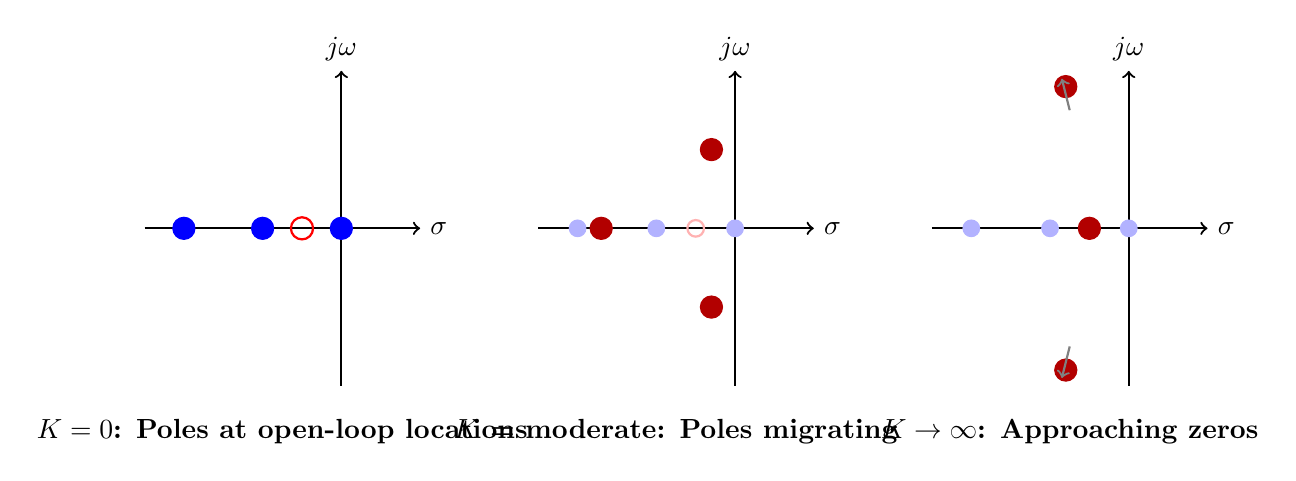
\begin{tikzpicture}[scale=1.0]
    % Before: K=0
    \begin{scope}[xshift=-5cm]
        \draw[->,thick] (-2.5,0) -- (1,0) node[right] {$\sigma$};
        \draw[->,thick] (0,-2) -- (0,2) node[above] {$j\omega$};

        \filldraw[blue] (-2,0) circle (4pt);
        \filldraw[blue] (-1,0) circle (4pt);
        \filldraw[blue] (0,0) circle (4pt);

        \draw[red,thick] (-0.5,0) circle (4pt);

        \node[below] at (-0.75,-2.3) {\textbf{$K = 0$: Poles at open-loop locations}};
    \end{scope}

    % After: K = medium
    \begin{scope}[xshift=0cm]
        \draw[->,thick] (-2.5,0) -- (1,0) node[right] {$\sigma$};
        \draw[->,thick] (0,-2) -- (0,2) node[above] {$j\omega$};

        % Original locations (faded)
        \filldraw[blue!30] (-2,0) circle (3pt);
        \filldraw[blue!30] (-1,0) circle (3pt);
        \filldraw[blue!30] (0,0) circle (3pt);
        \draw[red!30,thick] (-0.5,0) circle (3pt);

        % Current pole locations
        \filldraw[red!70!black] (-1.7,0) circle (4pt);
        \filldraw[red!70!black] (-0.3,1) circle (4pt);
        \filldraw[red!70!black] (-0.3,-1) circle (4pt);

        \node[below] at (-0.75,-2.3) {\textbf{$K$ = moderate: Poles migrating}};
    \end{scope}

    % After: K large
    \begin{scope}[xshift=5cm]
        \draw[->,thick] (-2.5,0) -- (1,0) node[right] {$\sigma$};
        \draw[->,thick] (0,-2) -- (0,2) node[above] {$j\omega$};

        % Original locations (faded)
        \filldraw[blue!30] (-2,0) circle (3pt);
        \filldraw[blue!30] (-1,0) circle (3pt);
        \filldraw[blue!30] (0,0) circle (3pt);
        \draw[red!30,thick] (-0.5,0) circle (3pt);

        % Current pole locations
        \filldraw[red!70!black] (-0.5,0) circle (4pt);
        \filldraw[red!70!black] (-0.8,1.8) circle (4pt);
        \filldraw[red!70!black] (-0.8,-1.8) circle (4pt);

        % Arrows showing direction
        \draw[->,thick,gray] (-0.75,1.5) -- (-0.85,1.9);
        \draw[->,thick,gray] (-0.75,-1.5) -- (-0.85,-1.9);

        \node[below] at (-0.75,-2.3) {\textbf{$K \to \infty$: Approaching zeros}};
    \end{scope}
\end{tikzpicture}
\caption{Pole migration as gain $K$ increases from zero to infinity. At $K=0$, closed-loop poles equal open-loop poles. As $K$ increases, poles migrate along the root locus branches toward zeros or infinity.}
\label{fig:pole_migration}
\end{figure}

\begin{figure}[H]
\centering
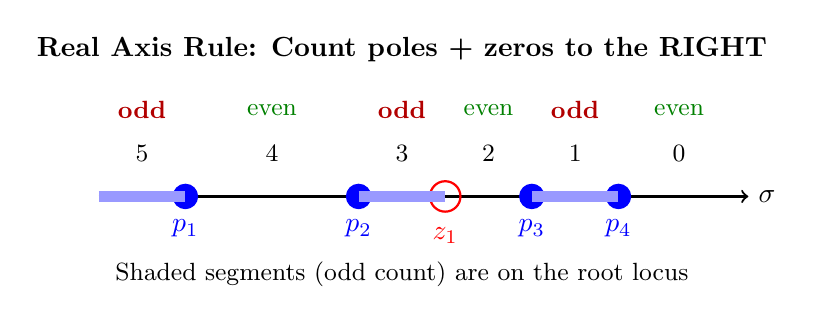
\begin{tikzpicture}[scale=1.1]
    % Real axis rule illustration
    \draw[->,thick] (-6,0) -- (1.5,0) node[right] {$\sigma$};

    % Poles and zeros
    \filldraw[blue] (-5,0) circle (4pt) node[below=5pt] {$p_1$};
    \filldraw[blue] (-3,0) circle (4pt) node[below=5pt] {$p_2$};
    \draw[red,thick] (-2,0) circle (5pt);
    \node[red,below] at (-2,-0.25) {$z_1$};
    \filldraw[blue] (-1,0) circle (4pt) node[below=5pt] {$p_3$};
    \filldraw[blue] (0,0) circle (4pt) node[below=5pt] {$p_4$};

    % Count indicators
    \node at (0.7,0.5) {\small 0};
    \node at (-0.5,0.5) {\small 1};
    \node at (-1.5,0.5) {\small 2};
    \node at (-2.5,0.5) {\small 3};
    \node at (-4,0.5) {\small 4};
    \node at (-5.5,0.5) {\small 5};

    % Odd/even labels
    \node[green!50!black] at (0.7,1) {\small even};
    \node[red!70!black] at (-0.5,1) {\small \textbf{odd}};
    \node[green!50!black] at (-1.5,1) {\small even};
    \node[red!70!black] at (-2.5,1) {\small \textbf{odd}};
    \node[green!50!black] at (-4,1) {\small even};
    \node[red!70!black] at (-5.5,1) {\small \textbf{odd}};

    % Root locus segments
    \draw[line width=4pt,blue!40] (-1,0) -- (0,0);
    \draw[line width=4pt,blue!40] (-3,0) -- (-2,0);
    \draw[line width=4pt,blue!40] (-6,0) -- (-5,0);

    % Header
    \node at (-2.5,1.7) {\textbf{Real Axis Rule: Count poles + zeros to the RIGHT}};
    \node at (-2.5,-0.9) {\small Shaded segments (odd count) are on the root locus};
\end{tikzpicture}
\caption{Illustration of the real axis segment rule. For each point on the real axis, count the total number of poles and zeros to its right. Segments where this count is odd belong to the root locus.}
\label{fig:real_axis_rule_detailed}
\end{figure}

%=============================================================================
\section{Summary}
\label{sec:summary}
%=============================================================================

The root locus method, developed by Walter Evans in 1948, provides a powerful graphical technique for analyzing how closed-loop poles move as gain varies. The key concepts encompass five main areas. The \textbf{fundamental equation} states that the root locus consists of all points satisfying $1 + KG(s)H(s) = 0$ for $K \geq 0$. The \textbf{angle criterion} establishes that a point lies on the root locus if $\angle G(s)H(s) = \pm 180°(2k+1)$. The \textbf{magnitude criterion} determines that once a point is confirmed on the locus, $K = 1/|G(s)H(s)|$. The \textbf{construction rules} provide eight guidelines for rapid sketching: branches start at poles and end at zeros or infinity; the locus is symmetric about the real axis; real axis segments occur to the left of an odd pole/zero count; asymptotes emanate at specified angles from the centroid; breakaway and break-in points occur where $dK/ds = 0$; and $j\omega$ crossings can be found from the Routh array. Finally, the \textbf{design application} involves selecting gain $K$ to place dominant poles in desired $s$-plane regions for required transient response characteristics.

While modern computational tools can generate root locus plots instantly, understanding the underlying principles enables engineers to predict how system modifications will affect closed-loop behavior, design compensators to reshape the locus favorably, develop intuition about dynamic system behavior, and verify computational results for correctness.

The root locus remains an indispensable tool in the control engineer's toolkit, bridging classical graphical methods with modern computational practice.

\newpage
%=============================================================================
\section{Exercises}
\label{sec:exercises}
%=============================================================================

\begin{exercise}
Sketch the root locus for $G(s) = \frac{K}{(s+1)(s+3)}$ and find the breakaway point.
\end{exercise}

\begin{exercise}
For $G(s) = \frac{K(s+4)}{s(s+1)(s+2)}$, determine the asymptotes and centroid.
\end{exercise}

\begin{exercise}
A unity feedback system has $G(s) = \frac{K}{s(s^2+6s+10)}$. Find the range of $K$ for stability.
\end{exercise}

\begin{exercise}
For $G(s) = \frac{K}{s(s+2)(s+4)}$, find the gain $K$ that places the dominant poles at $\zeta = 0.707$.
\end{exercise}

\begin{exercise}
Sketch the root locus for $G(s) = \frac{K(s+1)}{s^2(s+4)}$ and identify all key features.
\end{exercise}

\begin{exercise}
A system has the characteristic equation $s^3 + 3s^2 + (2+K)s + 4K = 0$. Sketch the root locus and find the imaginary axis crossing.
\end{exercise}

\begin{exercise}
Design a lead compensator to reshape the root locus of $G(s) = \frac{K}{s(s+2)}$ so that closed-loop poles with $\zeta = 0.5$ and $\omega_n = 4$ rad/s are achievable.
\end{exercise}

\begin{exercise}
Using MATLAB or Python, verify your hand-sketched root locus for Exercise 5 and determine the exact breakaway points numerically.
\end{exercise}

\begin{exercise}
For the transfer function $G(s) = \frac{K}{s(s+1)(s+5)}$, determine: (a) the number of asymptotes and their angles, (b) the centroid of the asymptotes, (c) the segments of the real axis that belong to the root locus, and (d) the range of $K$ for which the system is stable.
\end{exercise}

\begin{exercise}
A position control system has open-loop transfer function $G(s) = \frac{K(s+2)}{s^2(s+10)}$. Sketch the root locus and explain why this system has a break-in point. Find the break-in point location.
\end{exercise}

\begin{exercise}
Consider a system with $G(s)H(s) = \frac{K}{(s+1)^2(s+4)}$. Apply all eight root locus construction rules to sketch the complete locus. Mark the breakaway point and calculate the gain at which breakaway occurs.
\end{exercise}

\begin{exercise}
For the system $G(s) = \frac{K}{s(s^2+4s+8)}$, the complex poles are at $s = -2 \pm j2$. Using the angle criterion, determine whether the point $s = -3$ lies on the root locus.
\end{exercise}

%=============================================================================
% Bibliography would go here in a full document
%=============================================================================

